
%% bare_conf_compsoc.tex
%% V1.4b
%% 2015/08/26
%% by Michael Shell
%% See:
%% http://www.michaelshell.org/
%% for current contact information.
%%
%% This is a skeleton file demonstrating the use of IEEEtran.cls
%% (requires IEEEtran.cls version 1.8b or later) with an IEEE Computer
%% Society conference paper.
%%
%% Support sites:
%% http://www.michaelshell.org/tex/ieeetran/
%% http://www.ctan.org/pkg/ieeetran
%% and
%% http://www.ieee.org/

%%*************************************************************************
%% Legal Notice:
%% This code is offered as-is without any warranty either expressed or
%% implied; without even the implied warranty of MERCHANTABILITY or
%% FITNESS FOR A PARTICULAR PURPOSE! 
%% User assumes all risk.
%% In no event shall the IEEE or any contributor to this code be liable for
%% any damages or losses, including, but not limited to, incidental,
%% consequential, or any other damages, resulting from the use or misuse
%% of any information contained here.
%%
%% All comments are the opinions of their respective authors and are not
%% necessarily endorsed by the IEEE.
%%
%% This work is distributed under the LaTeX Project Public License (LPPL)
%% ( http://www.latex-project.org/ ) version 1.3, and may be freely used,
%% distributed and modified. A copy of the LPPL, version 1.3, is included
%% in the base LaTeX documentation of all distributions of LaTeX released
%% 2003/12/01 or later.
%% Retain all contribution notices and credits.
%% ** Modified files should be clearly indicated as such, including  **
%% ** renaming them and changing author support contact information. **
%%*************************************************************************


% *** Authors should verify (and, if needed, correct) their LaTeX system  ***
% *** with the testflow diagnostic prior to trusting their LaTeX platform ***
% *** with production work. The IEEE's font choices and paper sizes can   ***
% *** trigger bugs that do not appear when using other class files.       ***                          ***
% The testflow support page is at:
% http://www.michaelshell.org/tex/testflow/
\documentclass[conference,compsoc]{IEEEtran}
\makeatletter\if@twocolumn\PassOptionsToPackage{switch}{lineno}\else\fi\makeatother

\usepackage{graphicx}
\usepackage[T1]{fontenc}
% Some/most Computer Society conferences require the compsoc mode option,
% but others may want the standard conference format.
%
% If IEEEtran.cls has not been installed into the LaTeX system files,
% manually specify the path to it like:
% \documentclass[conference,compsoc]{../sty/IEEEtran}


% Some very useful LaTeX packages include:
% (uncomment the ones you want to load)


% *** MISC UTILITY PACKAGES ***
%
%\usepackage{ifpdf}
% Heiko Oberdiek's ifpdf.sty is very useful if you need conditional
% compilation based on whether the output is pdf or dvi.
% usage:
% \ifpdf
%   % pdf code
% \else
%   % dvi code
% \fi
% The latest version of ifpdf.sty can be obtained from:
% http://www.ctan.org/pkg/ifpdf
% Also, note that IEEEtran.cls V1.7 and later provides a builtin
% \ifCLASSINFOpdf conditional that works the same way.
% When switching from latex to pdflatex and vice-versa, the compiler may
% have to be run twice to clear warning/error messages.


% *** CITATION PACKAGES ***
%
\ifCLASSOPTIONcompsoc
  % IEEE Computer Society needs nocompress option
  % requires cite.sty v4.0 or later (November 2003)
  \usepackage[nocompress]{cite}
\else
  % normal IEEE
  \usepackage{cite}
\fi
% cite.sty was written by Donald Arseneau
% V1.6 and later of IEEEtran pre-defines the format of the cite.sty package
% \cite{} output to follow that of the IEEE. Loading the cite package will
% result in citation numbers being automatically sorted and properly
% "compressed/ranged". e.g., [1], [9], [2], [7], [5], [6] without using
% cite.sty will become [1], [2], [5]--[7], [9] using cite.sty. cite.sty's
% \cite will automatically add leading space, if needed. Use cite.sty's
% noadjust option (cite.sty V3.8 and later) if you want to turn this off
% such as if a citation ever needs to be enclosed in parenthesis.
% cite.sty is already installed on most LaTeX systems. Be sure and use
% version 5.0 (2009-03-20) and later if using hyperref.sty.
% The latest version can be obtained at:
% http://www.ctan.org/pkg/cite
% The documentation is contained in the cite.sty file itself.
%
% Note that some packages require special options to format as the Computer
% Society requires. In particular, Computer Society  papers do not use
% compressed citation ranges as is done in typical IEEE papers
% (e.g., [1]-[4]). Instead, they list every citation separately in order
% (e.g., [1], [2], [3], [4]). To get the latter we need to load the cite
% package with the nocompress option which is supported by cite.sty v4.0
% and later.


% *** GRAPHICS RELATED PACKAGES ***
%
\ifCLASSINFOpdf
  % \usepackage[pdftex]{graphicx}
  % declare the path(s) where your graphic files are
  % \graphicspath{{../pdf/}{../jpeg/}}
  % and their extensions so you won't have to specify these with
  % every instance of \includegraphics
  % \DeclareGraphicsExtensions{.pdf,.jpeg,.png}
\else
  % or other class option (dvipsone, dvipdf, if not using dvips). graphicx
  % will default to the driver specified in the system graphics.cfg if no
  % driver is specified.
  % \usepackage[dvips]{graphicx}
  % declare the path(s) where your graphic files are
  % \graphicspath{{../eps/}}
  % and their extensions so you won't have to specify these with
  % every instance of \includegraphics
  % \DeclareGraphicsExtensions{.eps}
\fi
% graphicx was written by David Carlisle and Sebastian Rahtz. It is
% required if you want graphics, photos, etc. graphicx.sty is already
% installed on most LaTeX systems. The latest version and documentation
% can be obtained at: 
% http://www.ctan.org/pkg/graphicx
% Another good source of documentation is "Using Imported Graphics in
% LaTeX2e" by Keith Reckdahl which can be found at:
% http://www.ctan.org/pkg/epslatex
%
% latex, and pdflatex in dvi mode, support graphics in encapsulated
% postscript (.eps) format. pdflatex in pdf mode supports graphics
% in .pdf, .jpeg, .png and .mps (metapost) formats. Users should ensure
% that all non-photo figures use a vector format (.eps, .pdf, .mps) and
% not a bitmapped formats (.jpeg, .png). The IEEE frowns on bitmapped formats
% which can result in "jaggedy"/blurry rendering of lines and letters as
% well as large increases in file sizes.
%
% You can find documentation about the pdfTeX application at:
% http://www.tug.org/applications/pdftex


% *** MATH PACKAGES ***
%
\usepackage{amsmath}
\usepackage[cmintegrals]{newtxmath}
% A popular package from the American Mathematical Society that provides
% many useful and powerful commands for dealing with mathematics.
%
% Note that the amsmath package sets \interdisplaylinepenalty to 10000
% thus preventing page breaks from occurring within multiline equations. Use:
\interdisplaylinepenalty=2500
% after loading amsmath to restore such page breaks as IEEEtran.cls normally
% does. amsmath.sty is already installed on most LaTeX systems. The latest
% version and documentation can be obtained at:
% http://www.ctan.org/pkg/amsmath


% *** SPECIALIZED LIST PACKAGES ***
%
%\usepackage{algorithmic}
% algorithmic.sty was written by Peter Williams and Rogerio Brito.
% This package provides an algorithmic environment fo describing algorithms.
% You can use the algorithmic environment in-text or within a figure
% environment to provide for a floating algorithm. Do NOT use the algorithm
% floating environment provided by algorithm.sty (by the same authors) or
% algorithm2e.sty (by Christophe Fiorio) as the IEEE does not use dedicated
% algorithm float types and packages that provide these will not provide
% correct IEEE style captions. The latest version and documentation of
% algorithmic.sty can be obtained at:
% http://www.ctan.org/pkg/algorithms
% Also of interest may be the (relatively newer and more customizable)
% algorithmicx.sty package by Szasz Janos:
% http://www.ctan.org/pkg/algorithmicx


% *** ALIGNMENT PACKAGES ***
%
%\usepackage{array}
% Frank Mittelbach's and David Carlisle's array.sty patches and improves
% the standard LaTeX2e array and tabular environments to provide better
% appearance and additional user controls. As the default LaTeX2e table
% generation code is lacking to the point of almost being broken with
% respect to the quality of the end results, all users are strongly
% advised to use an enhanced (at the very least that provided by array.sty)
% set of table tools. array.sty is already installed on most systems. The
% latest version and documentation can be obtained at:
% http://www.ctan.org/pkg/array


% IEEEtran contains the IEEEeqnarray family of commands that can be used to
% generate multiline equations as well as matrices, tables, etc., of high
% quality.


% *** SUBFIGURE PACKAGES ***
%\ifCLASSOPTIONcompsoc
%  \usepackage[caption=false,font=footnotesize,labelfont=sf,textfont=sf]{subfig}
%\else
%  \usepackage[caption=false,font=footnotesize]{subfig}
%\fi
% subfig.sty, written by Steven Douglas Cochran, is the modern replacement
% for subfigure.sty, the latter of which is no longer maintained and is
% incompatible with some LaTeX packages including fixltx2e. However,
% subfig.sty requires and automatically loads Axel Sommerfeldt's caption.sty
% which will override IEEEtran.cls' handling of captions and this will result
% in non-IEEE style figure/table captions. To prevent this problem, be sure
% and invoke subfig.sty's "caption=false" package option (available since
% subfig.sty version 1.3, 2005/06/28) as this is will preserve IEEEtran.cls
% handling of captions.
% Note that the Computer Society format requires a sans serif font rather
% than the serif font used in traditional IEEE formatting and thus the need
% to invoke different subfig.sty package options depending on whether
% compsoc mode has been enabled.
%
% The latest version and documentation of subfig.sty can be obtained at:
% http://www.ctan.org/pkg/subfig


% *** FLOAT PACKAGES ***
%
%\usepackage{fixltx2e}
% fixltx2e, the successor to the earlier fix2col.sty, was written by
% Frank Mittelbach and David Carlisle. This package corrects a few problems
% in the LaTeX2e kernel, the most notable of which is that in current
% LaTeX2e releases, the ordering of single and double column floats is not
% guaranteed to be preserved. Thus, an unpatched LaTeX2e can allow a
% single column figure to be placed prior to an earlier double column
% figure.
% Be aware that LaTeX2e kernels dated 2015 and later have fixltx2e.sty's
% corrections already built into the system in which case a warning will
% be issued if an attempt is made to load fixltx2e.sty as it is no longer
% needed.
% The latest version and documentation can be found at:
% http://www.ctan.org/pkg/fixltx2e


%\usepackage{stfloats}
% stfloats.sty was written by Sigitas Tolusis. This package gives LaTeX2e
% the ability to do double column floats at the bottom of the page as well
% as the top. (e.g., "\begin{figure*}[!b]" is not normally possible in
% LaTeX2e). It also provides a command:
%\fnbelowfloat
% to enable the placement of footnotes below bottom floats (the standard
% LaTeX2e kernel puts them above bottom floats). This is an invasive package
% which rewrites many portions of the LaTeX2e float routines. It may not work
% with other packages that modify the LaTeX2e float routines. The latest
% version and documentation can be obtained at:
% http://www.ctan.org/pkg/stfloats
% Do not use the stfloats baselinefloat ability as the IEEE does not allow
% \baselineskip to stretch. Authors submitting work to the IEEE should note
% that the IEEE rarely uses double column equations and that authors should try
% to avoid such use. Do not be tempted to use the cuted.sty or midfloat.sty
% packages (also by Sigitas Tolusis) as the IEEE does not format its papers in
% such ways.
% Do not attempt to use stfloats with fixltx2e as they are incompatible.
% Instead, use Morten Hogholm'a dblfloatfix which combines the features
% of both fixltx2e and stfloats:
%
% \usepackage{dblfloatfix}
% The latest version can be found at:
% http://www.ctan.org/pkg/dblfloatfix


% *** PDF, URL AND HYPERLINK PACKAGES ***
%
%\usepackage{url}
% url.sty was written by Donald Arseneau. It provides better support for
% handling and breaking URLs. url.sty is already installed on most LaTeX
% systems. The latest version and documentation can be obtained at:
% http://www.ctan.org/pkg/url
% Basically, \url{my_url_here}.


% *** Do not adjust lengths that control margins, column widths, etc. ***
% *** Do not use packages that alter fonts (such as pslatex).         ***
% There should be no need to do such things with IEEEtran.cls V1.6 and later.
% (Unless specifically asked to do so by the journal or conference you plan
% to submit to, of course. )


% correct bad hyphenation here
\hyphenation{op-tical net-works semi-conduc-tor}

%%%%%%%%%%%%%%%%%%%%%%%%%%%%%%%%%%%%%%%%%%%%%%%%%%%%%%%%%%%%%%%%%%%%%%%%%%
% Following additional macros are required to function some 
% functions which are not available in the class used.
%%%%%%%%%%%%%%%%%%%%%%%%%%%%%%%%%%%%%%%%%%%%%%%%%%%%%%%%%%%%%%%%%%%%%%%%%%
\usepackage{url,multirow,morefloats,floatflt,cancel,tfrupee}
\makeatletter


\AtBeginDocument{\@ifpackageloaded{textcomp}{}{\usepackage{textcomp}}}
\makeatother
\usepackage{colortbl}
\usepackage{xcolor}
\usepackage{pifont}
\usepackage[nointegrals]{wasysym}
\urlstyle{rm}
\makeatletter

%%%For Table column width calculation.
\def\mcWidth#1{\csname TY@F#1\endcsname+\tabcolsep}

%%Hacking center and right align for table
\def\cAlignHack{\rightskip\@flushglue\leftskip\@flushglue\parindent\z@\parfillskip\z@skip}
\def\rAlignHack{\rightskip\z@skip\leftskip\@flushglue \parindent\z@\parfillskip\z@skip}

%Etal definition in references
\@ifundefined{etal}{\def\etal{\textit{et~al}}}{}


%\if@twocolumn\usepackage{dblfloatfix}\fi
\usepackage{ifxetex}
\ifxetex\else\if@twocolumn\@ifpackageloaded{stfloats}{}{\usepackage{dblfloatfix}}\fi\fi

\AtBeginDocument{
\expandafter\ifx\csname eqalign\endcsname\relax
\def\eqalign#1{\null\vcenter{\def\\{\cr}\openup\jot\m@th
  \ialign{\strut$\displaystyle{##}$\hfil&$\displaystyle{{}##}$\hfil
      \crcr#1\crcr}}\,}
\fi
}

%For fixing hardfail when unicode letters appear inside table with endfloat
\AtBeginDocument{%
  \@ifpackageloaded{endfloat}%
   {\renewcommand\efloat@iwrite[1]{\immediate\expandafter\protected@write\csname efloat@post#1\endcsname{}}}{\newif\ifefloat@tables}%
}%

\def\BreakURLText#1{\@tfor\brk@tempa:=#1\do{\brk@tempa\hskip0pt}}
\let\lt=<
\let\gt=>
\def\processVert{\ifmmode|\else\textbar\fi}
\let\processvert\processVert

\@ifundefined{subparagraph}{
\def\subparagraph{\@startsection{paragraph}{5}{2\parindent}{0ex plus 0.1ex minus 0.1ex}%
{0ex}{\normalfont\small\itshape}}%
}{}

% These are now gobbled, so won't appear in the PDF.
\newcommand\role[1]{\unskip}
\newcommand\aucollab[1]{\unskip}
  
\@ifundefined{tsGraphicsScaleX}{\gdef\tsGraphicsScaleX{1}}{}
\@ifundefined{tsGraphicsScaleY}{\gdef\tsGraphicsScaleY{.9}}{}
% To automatically resize figures to fit inside the text area
\def\checkGraphicsWidth{\ifdim\Gin@nat@width>\linewidth
	\tsGraphicsScaleX\linewidth\else\Gin@nat@width\fi}

\def\checkGraphicsHeight{\ifdim\Gin@nat@height>.9\textheight
	\tsGraphicsScaleY\textheight\else\Gin@nat@height\fi}

\def\fixFloatSize#1{}%\@ifundefined{processdelayedfloats}{\setbox0=\hbox{\includegraphics{#1}}\ifnum\wd0<\columnwidth\relax\renewenvironment{figure*}{\begin{figure}}{\end{figure}}\fi}{}}
\let\ts@includegraphics\includegraphics

\def\inlinegraphic[#1]#2{{\edef\@tempa{#1}\edef\baseline@shift{\ifx\@tempa\@empty0\else#1\fi}\edef\tempZ{\the\numexpr(\numexpr(\baseline@shift*\f@size/100))}\protect\raisebox{\tempZ pt}{\ts@includegraphics{#2}}}}

%\renewcommand{\includegraphics}[1]{\ts@includegraphics[width=\checkGraphicsWidth]{#1}}
\AtBeginDocument{\def\includegraphics{\@ifnextchar[{\ts@includegraphics}{\ts@includegraphics[width=\checkGraphicsWidth,height=\checkGraphicsHeight,keepaspectratio]}}}

\DeclareMathAlphabet{\mathpzc}{OT1}{pzc}{m}{it}

\def\URL#1#2{\@ifundefined{href}{#2}{\href{#1}{#2}}}

%%For url break
\def\UrlOrds{\do\*\do\-\do\~\do\'\do\"\do\-}%
\g@addto@macro{\UrlBreaks}{\UrlOrds}



\edef\fntEncoding{\f@encoding}
\def\EUoneEnc{EU1}
\makeatother
\def\floatpagefraction{0.8} 
\def\dblfloatpagefraction{0.8}
\def\style#1#2{#2}
\def\xxxguillemotleft{\fontencoding{T1}\selectfont\guillemotleft}
\def\xxxguillemotright{\fontencoding{T1}\selectfont\guillemotright}

\newif\ifmultipleabstract\multipleabstractfalse%
\newenvironment{typesetAbstractGroup}{}{}%

%%%%%%%%%%%%%%%%%%%%%%%%%%%%%%%%%%%%%%%%%%%%%%%%%%%%%%%%%%%%%%%%%%%%%%%%%%
\usepackage{tabulary}
\makeatletter
\AtBeginDocument{\@ifpackageloaded{longtable}{%
\def\LT@makecaption#1#2#3{%
  \LT@mcol\LT@cols c{\hbox to\z@{\hss\parbox[t]\LTcapwidth{%
    \sbox\@tempboxa{#1{#2: } #3}%
    \ifdim\wd\@tempboxa>\hsize
      #1{#2: }\textsc{#3}%
    \else
      \hbox to\hsize{\hfil\box\@tempboxa\hfil}%
    \fi
    \endgraf\vskip\baselineskip}%
  \hss}}}
}{}}
\makeatother

\makeatletter
\let\citep\cite
\let\citet\cite
\makeatother


\makeatletter
\def\fig@textbf{\textbf}
\AtBeginDocument{\renewcommand\floatc@plain[2]{\setbox\@tempboxa\hbox{{\footnotesize#1.}\footnotesize\hskip.5em#2}%
\ifdim\wd\@tempboxa>\hsize {\fig@textbf{\footnotesize#1.}}\footnotesize\hskip.5em#2\par
\else\hbox to\hsize{\hfil\box\@tempboxa\hfil}\fi}}
\makeatother
  
\def\THEYEAR{2016}
%%%%%%%%%%%%%%%%%%%%%%%%%%%%%%%%%%%%%%%%%%
% Feature enabled:
%full-reference: true

\usepackage{float}

\begin{document}

\nocite{*}


%
% paper title
% Titles are generally capitalized except for words such as a, an, and, as,
% at, but, by, for, in, nor, of, on, or, the, to and up, which are usually
% not capitalized unless they are the first or last word of the title.
% Linebreaks \\ can be used within to get better formatting as desired.
% Do not put math or special symbols in the title.

% conference papers do not typically use \thanks and this command
% is locked out in conference mode. If really needed, such as for
% the acknowledgment of grants, issue a \IEEEoverridecommandlockouts
% after \documentclass

\title{Drive-Net: Convolutional Network for Driver Distraction Detection}
      
% author names and affiliations
% use a multiple column layout for up to three different
% affiliations
\author{
    \IEEEauthorblockN{{Mohammed S.~Majdi}\IEEEauthorrefmark{1}, 
          {Sundaresh~Ram}\IEEEauthorrefmark{2}, 
          {Jonathan T~Gill}\IEEEauthorrefmark{1}, 
          {Jeffrey J~Rodriguez}\IEEEauthorrefmark{1}}
    \IEEEauthorblockA{\IEEEauthorrefmark{1}Electrical and Computer Engineering, \\University of Arizona, AZ, Tucson, USA}
    \IEEEauthorblockA{\IEEEauthorrefmark{2}School of Electrical and Computer Engineering, \\Cornell University, NY, Ithaca, USA}\\Email: mohammadsmajdi@arizona.edu ({Mohammed S.~Majdi})\\Email: sr2255@cornel.edu ({Sundaresh~Ram})\\Email: jtgill@arizona.edu ({Jonathan T~Gill})\\Email: jjrodrig@arizona.edu ({Jeffrey J~Rodriguez})}
% use for special paper notices
%\IEEEspecialpapernotice{(Invited Paper)}

% make the title area

\maketitle 
% As a general rule, do not put math, special symbols or citations
% in the abstract or keywords.

\begin{abstract}
To help prevent motor vehicle accidents, there has been significant interest in finding an automated method to recognize signs of driver distraction, such as talking to passengers, fixing hair and makeup, eating and drinking, and using a cell phone. In this paper, we present an automated supervised learning method called Drive-Net for driver distraction detection. Drive-Net uses a combination of a convolutional neural network (CNN) and a random decision forest to classify images of a driver. We compare the performance of our proposed Drive-Net to two other popular machine learning approaches: a recurrent neural network (RNN) and a multilayer perceptron (MLP). We tested the methods on a publicly available database of images acquired in a controlled environment that contained about 22425 images manually annotated by an expert. The results show that Drive-Net achieves a detection accuracy of 95\%, which is 2\% more than the best results obtained in the same database using other methods.
\end{abstract}
    
% Note that keywords are not normally used for peerreview papers.

\begin{IEEEkeywords}Image classification, convolutional neural networks, random forest, driver distraction\end{IEEEkeywords}
% For peer review papers, you can put extra information on the cover
% page as needed:
% \ifCLASSOPTIONpeerreview
% \begin{center} \bfseries EDICS Category: 3-BBND \end{center}
% \fi
%
% For peerreview papers, this IEEEtran command inserts a page break and
% creates the second title. It will be ignored for other modes.
\IEEEpeerreviewmaketitle


% An example of a floating figure using the graphicx package.
% Note that \label must occur AFTER (or within) \caption.
% For figures, \caption should occur after the \includegraphics.
% Note that IEEEtran v1.7 and later has special internal code that
% is designed to preserve the operation of \label within \caption
% even when the captionsoff option is in effect. However, because
% of issues like this, it may be the safest practice to put all your
% \label just after \caption rather than within \caption{}.
%
% Reminder: the "draftcls" or "draftclsnofoot", not "draft", class
% option should be used if it is desired that the figures are to be
% displayed while in draft mode.
%
%\begin{figure}[!t]
%\centering
%\includegraphics[width=2.5in]{myfigure}
% where an .eps filename suffix will be assumed under latex, 
% and a .pdf suffix will be assumed for pdflatex; or what has been declared
% via \DeclareGraphicsExtensions.
%\caption{Simulation results for the network.}
%\label{fig_sim}
%\end{figure}

% Note that the IEEE typically puts floats only at the top, even when this
% results in a large percentage of a column being occupied by floats.


% An example of a double column floating figure using two subfigures.
% (The subfig.sty package must be loaded for this to work.)
% The subfigure \label commands are set within each subfloat command,
% and the \label for the overall figure must come after \caption.
% \hfil is used as a separator to get equal spacing.
% Watch out that the combined width of all the subfigures on a 
% line do not exceed the text width or a line break will occur.
%
%\begin{figure*}[!t]
%\centering
%\subfloat[Case I]{\includegraphics[width=2.5in]{box}%
%\label{fig_first_case}}
%\hfil
%\subfloat[Case II]{\includegraphics[width=2.5in]{box}%
%\label{fig_second_case}}
%\caption{Simulation results for the network.}
%\label{fig_sim}
%\end{figure*}
%
% Note that often IEEE papers with subfigures do not employ subfigure
% captions (using the optional argument to \subfloat[]), but instead will
% reference/describe all of them (a), (b), etc., within the main caption.
% Be aware that for subfig.sty to generate the (a), (b), etc., subfigure
% labels, the optional argument to \subfloat must be present. If a
% subcaption is not desired, just leave its contents blank,
% e.g., \subfloat[].


% An example of a floating table. Note that, for IEEE style tables, the
% \caption command should come BEFORE the table and, given that table
% captions serve much like titles, are usually capitalized except for words
% such as a, an, and, as, at, but, by, for, in, nor, of, on, or, the, to
% and up, which are usually not capitalized unless they are the first or
% last word of the caption. Table text will default to \footnotesize as
% the IEEE normally uses this smaller font for tables.
% The \label must come after \caption as always.
%
%\begin{table}[!t]
%% increase table row spacing, adjust to taste
%\renewcommand{\arraystretch}{1.3}
% if using array.sty, it might be a good idea to tweak the value of
% \extrarowheight as needed to properly center the text within the cells
%\caption{An Example of a Table}
%\label{table_example}
%\centering
%% Some packages, such as MDW tools, offer better commands for making tables
%% than the plain LaTeX2e tabular which is used here.
%\begin{tabular}{|c||c|}
%\hline
%One & Two\\
%\hline
%Three & Four\\
%\hline
%\end{tabular}
%\end{table}


% Note that the IEEE does not put floats in the very first column
% - or typically anywhere on the first page for that matter. Also,
% in-text middle ("here") positioning is typically not used, but it
% is allowed and encouraged for Computer Society conferences (but
% not Computer Society journals). Most IEEE journals/conferences use
% top floats exclusively. 
% Note that, LaTeX2e, unlike IEEE journals/conferences, places
% footnotes above bottom floats. This can be corrected via the
% \fnbelowfloat command of the stfloats package.


\section{Introduction}
Distracted driving is a major cause of motor vehicle accidents. Each day in the United States, approximately 9 people are killed and more than 1000 are injured in crashes that involve a distracted driver. \unskip~\cite{1641075:26775855} It is estimated that about 25\% of fatalities in motor vehicle accidents are due to distracted driving. \unskip~\cite{1641075:26775848} A study of American motor vehicle fatalities \unskip~\cite{1641075:26775855} reveals the top 10 causes of distracted driving:


  
  \begin{enumerate}
  \item \relax Generally distracted or ``lost in thought'' -{\textendash} 62\%
  \item \relax Cell phone use {\textemdash} 12\%
  \item \relax Outside person, object, or event {\textendash} 7\%.
  \item \relax Other occupants -{\textendash} 5\%.
  \item \relax Using or reaching for a device brought into the car (e.g., phone) {\textendash} 2\%.
  \item \relax Eating or drinking -{\textendash} 2\%.
  \item \relax Adjusting audio or climate controls {\textemdash} 2\%.
  \item \relax Using devices to operate the vehicle (e.g., adjusting mirrors or seatbelts) {\textemdash} 1\%.
  \item \relax Moving objects (e.g., insects or pets) -{\textendash} 1\%
  \item \relax Smoking related {\textemdash} 1\%.
  \end{enumerate}
  
  Therefore, there is interest in using dashboard camera image analysis to automatically detect drivers engaged in distracting behavior. A dataset of such dashboard camera images, observing various activities of drivers, has been compiled and used for the Kaggle competition regarding automated detection of driver distraction. \unskip~\cite{1641075:26775858} Figure~\ref{Drive-Net/figure1} shows examples of some images from the dashboard camera manually annotated as different activities while driving.


\bgroup
\fixFloatSize{Drive-Net/figures/image1.jpeg}
\begin{figure*}[!htbp]
\centering 
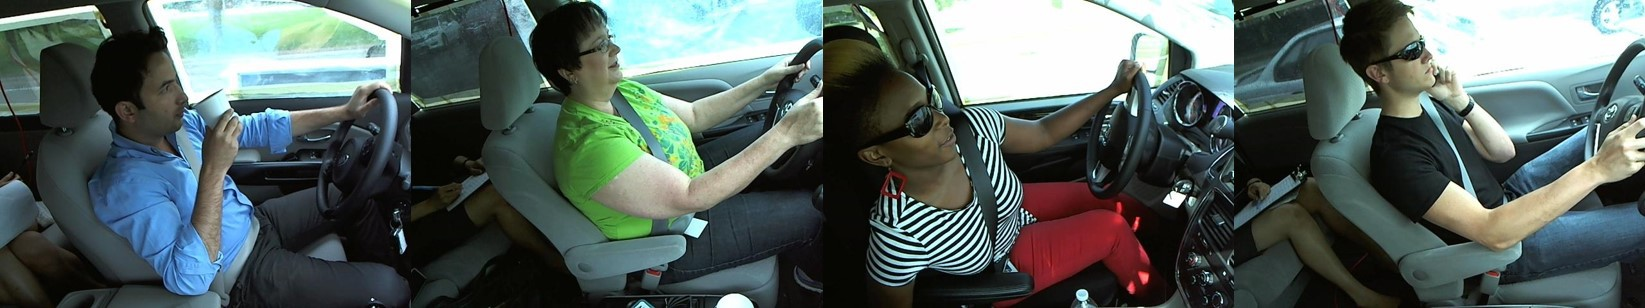
\includegraphics{Drive-Net/figures/image1.jpeg}
\caption{Representative dashboard camera images of drivers being distracted. From left to right: drinking while driving; safe driving; reaching behind while driving; talking on the phone (left hand) while driving. \unskip~\protect\cite{1641075:26775858}}
\label{Drive-Net/figure1}
\end{figure*}
\egroup

Object detection and human behavior detection are well-researched topics in the computer vision literature. \unskip~\cite{1641075:26775854} Machine learning (esp. Deep Learning) techniques can often learn complex models and achieve high accuracy, so many researchers have started to apply such techniques to solve computer vision problems, including object detection and human behavior detection. For example, the Inception-v4 model proposed by Szegedy \unskip~\cite{1641075:26775859} is a supervised learning model made up of deep convolutional residual networks (ResNet) that have more than 75 trainable layers, and achieves 96.92\% accuracy in the ImageNet data set. Girshick \unskip~\cite{1641075:26775856} introduced a very powerful method for object detection and segmentation using a region-based convolutional neural network (CNN). This method divides the human behavior detection problem into two problems. First, they apply an object detection algorithm to detect the regions of interest (ROIs) where people are present within an image. Next, each ROI is fed to a CNN to identify the type of behavior exhibited in the given ROI. Adding other traditional machine learning methods, such as ensemble learning (i.e. bagging) and K nearest neighbors (KNN), to the CNN model is a way to improve the accuracy of the already existing model. \unskip~\cite{1641075:26775847}

\bgroup
\begin{figure*}[!htbp]
\centering 
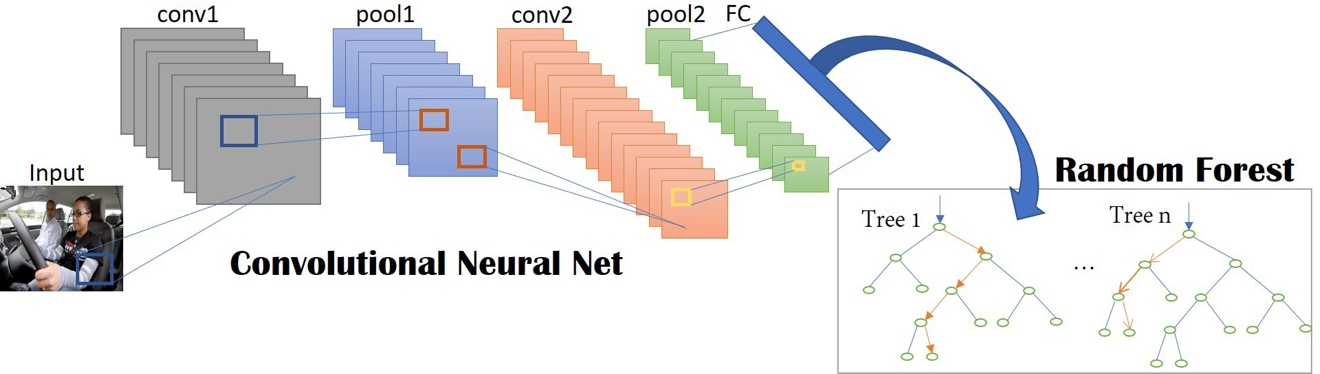
\includegraphics{Drive-Net/figures/image2.jpeg}
\caption{An overview of the proposed Drive-Net. Our proposed CNN architecture (shown on the left side) consists of two convolution layers (conv), each followed by a maxpooling layer (pool), and a final ReLU layer, the output of which is regularized using dropouts to obtain a fully connected layer (FC). The FC layer is fed as input to the random forest classifier (on the right side), which predicts the final class label.}
\label{Drive-Net/figure2}
\end{figure*}
\egroup

One of the main drawbacks of CNN is that training the network using a large data set can lead to overfitting the model. To avoid this, ensemble methods such as random decision forests can be effective. With this in mind, we propose a new supervised learning algorithm called Drive-Net that combines a CNN and a random forest in a cascading fashion for application to the problem of driver distraction detection using dashboard camera images. We compare our proposed Drive-Net to two other neural network methods: a residual neural network (RNN) and a multilayer perceptron (MLP). We show that Drive-Net achieves better classification accuracy than the driver distraction detection algorithms that were proposed in the Kaggle competition. \unskip~\cite{1641075:26775858}
    
\section{Methods}
Our proposed method, Drive-Net, is a cascaded classifier consisting of two stages: a CNN as the first stage, whose output layer is fed as input to a random decision forest to predict the final class label. We define each stage in detail below.



\subsection{Convolutional Neural Network Configurations} We adopted the U-Net architecture \unskip~\cite{1641075:26775850} as the basis for our CNN. The motivation behind this architecture is that the contracting path captures the context around the objects to provide a better representation of the object compared to architectures such as AlexNet \unskip~\cite{1641075:26775852} and VGGNet \unskip~\cite{1641075:26775860} Very large networks like AlexNet and VGGNet require learning a massive number of parameters and are very difficult to train in general, needing significant computational time. Thus, we empirically modified the U-Net architecture in this work to suit our application.

To construct our CNN, we discard U-Net's layers of up-convolution and the last two layers of down-sampling and replace them with a $1\times1 $ convolution instead to obtain a fully connected layer. We use the rectifier activation function \unskip~\cite{1641075:26775860} for our CNN as the constant gradient of rectified linear units (ReLU) results in faster learning and reduces the problem of vanishing gradient compared to the hyperbolic tangent (${{tanh}{\left(\bullet\right)}} $). We implement a maximum-pooling layer instead of average-pooling in the subsampling layer. We observed that the performance is better when a ReLU layer was configured with the maximum pool layer, resulting in higher classification accuracy after 50 epochs. We use the $1\times1 $ convolutional filter for the Adam \unskip~\cite{1641075:26775857} optimizer. All other parameters, such as the number of layers, the size of the convolutional kernel, the training algorithm, and the number of neurons in the final dense layer, were experimentally determined for our application.

To keep the training time small, we reduced the size of the dashboard camera images by a factor of 10 by making them 64 \ensuremath{\times} 48 in size and feed them as input to our CNN. We do not zero-pad the image patches, as the ROI of human activity is located toward the center of the image. Two consecutive convolutional layers are used in the network. The first convolutional layer consists of 32 kernels of size $5\times5\times1 $. The second convolutional layer consists of 64 kernels of size $5\times5\times32 $. The subsampling layer is set as the maximum value in nonoverlapping windows of size $2\times2 $ (stride of 2). This reduces the size of the output of each convolutional layer by half. After the two convolutional and subsampling layers, we use a ReLU layer, where the activation y for a given input x is obtained as
\let\saveeqnno\theequation
\let\savefrac\frac
\def\dispfrac{\displaystyle\savefrac}
\begin{eqnarray}
\let\frac\dispfrac
\gdef\theequation{1}
\let\theHequation\theequation
\label{disp-formula-group-e98e45e883854b6aa2d919dcc0573fee}
\begin{array}{@{}l}y=f\left(x\right)=\text{max}(0,x)\end{array}
\end{eqnarray}
\global\let\theequation\saveeqnno
\addtocounter{equation}{-1}\ignorespaces 
A graphical representation of the architecture of the proposed CNN model is shown in Figure~\ref{Drive-Net/figure2}  (see the left side).


\subsection{Random Decision Forest}A random forest classifier consists of a collection of decision tree classifiers combined to predict the class label, where each tree is grown in a randomized fashion. Each decision tree classifier consists of decision (or split) nodes and prediction (or leaf) nodes. The prediction nodes of each tree in the random forest classifier are labeled by the posterior distribution over the image classes. \unskip~\cite{1641075:26775861} Each decision node contains a test that best splits the space of the data to be classified. An image is classified by sending it down the decision tree and aggregating the posterior distributions that are reached. Most of the time, randomness is added to training at two points: when subsampling the training data and when choosing node tests. Each tree within the random forest classifier is binary and grows top-down. At each node, we select the binary test to maximize the information gain obtained by partitioning the training set $Q$ of image patches into two sets $Q_i$ according to the test.

\let\saveeqnno\theequation
\let\savefrac\frac
\def\dispfrac{\displaystyle\savefrac}
\begin{eqnarray}
\let\frac\dispfrac
\gdef\theequation{2}
\let\theHequation\theequation
\label{disp-formula-group-d27d73835da3454a817782924579e245}
\begin{array}{@{}l}\Delta E=-{\sum_i{\frac{\left(Q_i\right\vert}{\left(Q\right\vert}E\left(Q_i\right)}}\end{array}
\end{eqnarray}
\global\let\theequation\saveeqnno
\addtocounter{equation}{-1}\ignorespaces 

Here $E\left(\cdot\right) $\ensuremath{_{}}is the entropy of the set and $\left\vert \cdot\right\vert $\ensuremath{_{}}is the size of the set. We repeat this selection process for each decision node until it reaches a certain depth. Many implementations of random forests \unskip~\cite{1641075:26775846}, \unskip~\cite{1641075:26775849} use simple pixel-level tests at the nodes because it results in faster tree convergence. As we are interested in features that encode shape and appearance, we are interested in spatial correspondence between pixels. Therefore, we use a simple test proposed by Bosch \unskip~\cite{1641075:26775861} {\textemdash} as a linear classifier on the characteristic vector {\textemdash} at each decision node.

Suppose that $T $ is the set of all trees, $C $ is the set of all classes, and $L $ is the set of all leaves for a given tree. During training, posterior probabilities $P_{t,l}\left(Y\left(I\right)=c\:\right) $ for each class $c\in C $ are found at each leaf node $l\in L $ for each tree $t\in T $. These probabilities are calculated as the ratio of the number of images $I $ of class $c $ that reach a leaf node $l $ to the total number of images that reach that leaf node $l $. $Y\left(I\right) $ is the class label of image $I $. During test time, we pass a new image through every decision tree until it reaches a prediction (or leaf) node, average all the posterior probabilities, and classify the image as

\let\saveeqnno\theequation
\let\savefrac\frac
\def\dispfrac{\displaystyle\savefrac}
\begin{eqnarray}
\let\frac\dispfrac
\gdef\theequation{3}
\let\theHequation\theequation
\label{disp-formula-group-032e1395024b44bca0feeb46474c0adc}
\begin{array}{@{}l}\widehat Y\left(I\right)=\underset c{\text{argmax}}\left\{\frac1{\left\vert T\right\vert}\sum_{t=1}^{\left\vert T\right\vert}P_{t,l}\left(Y\left(I\right)=c\right)\right\}\end{array}
\end{eqnarray}
\global\let\theequation\saveeqnno
\addtocounter{equation}{-1}\ignorespaces 

where $l $ is the leaf node reached by the image $I $ in the tree $t $. A graphical representation of the proposed random forest classifier is shown in Figure~\ref{Drive-Net/figure2}  (see the right side).
    
\section{Experiments and Results}


\subsection{Data set} The Kaggle competition \unskip~\cite{1641075:26775858} for driver distraction has provided 22425 images for training and 79727 for tests. Since we did not have access to the test labels, our experiments were done solely on the training images. However, the quality and conditions of the training and testing images are similar; the only difference is that none of the drivers used in the training data set appear in the images in the test data set. The images are of size 640 \ensuremath{\times} 480, and for our experiments we converted them from color to grayscale.

Ten classes are provided, related to the ones listed in Section I. Each class includes almost tens of the data, so that we have a uniform distribution of sample data.

\begin{itemize}
  \item \relax c0: safe driving
  \item \relax c1: texting (right hand)
  \item \relax c2: talking on the phone (right hand)
  \item \relax c3: texting (left hand)
  \item \relax c4: talking on the phone (left hand)
  \item \relax c5: operating the radio
  \item \relax c6: drinking
  \item \relax c7: reaching behind
  \item \relax c8: hair and makeup
  \item \relax c9: talking to a passenger
\end{itemize}
  


\subsection{Algorithm Parameters}The convolutional neural random forest classifier is implemented using TensorFlow, \unskip~\cite{1641075:26775853} and runs on an NVIDIA GeForce GTX TITAN X GPU with 16 GB of memory. The classifier was trained using the Adam stochastic gradient descent algorithm \unskip~\cite{1641075:26775857} to efficiently optimize CNN weights. The weights were normalized using initialization as proposed in Kingma \unskip~\cite{1641075:26775857} and updated in a mini-batch scheme of 128 candidates. The biases were initialized with zero and the learning rate was set at $\alpha\;=\;0.001 $. The exponential decay rates for the estimates for the first and second moments were set as $\beta_1\;=\;0.9 $ and $\beta_2\;=\;0.99 $, respectively. We used $\epsilon={10}^{-8} $ to prevent division by zero. A dropout rate of $0.5 $ was implemented as regularization, applied to the output of the last convolutional layer and the dense layer to avoid overfitting. Finally, we used an epoch size of 50.  SoftMax loss (cross-entropy error loss) was used to measure the error loss. We used 100 estimators and a keep rate of $\gamma\;=\;{10}^{-4} $ for the random forest algorithm.


\subsection{Performance Evaluation} We tested the algorithm performance by performing k-fold cross-validation on the entire dataset. For our experiments, we varied the values of $k\in\lbrack2,\;5\rbrack $ and found that the results were consistent enough to indicate that the network is not overfitting. Therefore, we chose $k\;=\;5 $. First, we randomly choose the order of the driver images within the data set. For each fold of the k-fold cross-validation, we chose 80\% of the 22425 images as the training data set and tested the trained model on the remaining 20\% of the images. We ensured that the images from the entire dataset appeared in the test dataset only once in all k-folds, thereby allowing each image to be classified as a test image exactly once.

We compared our proposed Drive-Net with two other neural network classifiers: an RNN classifier, \unskip~\cite{1641075:26775863} and an MLP classifier \unskip~\cite{1641075:26775862}. We report the classification accuracy, which is defined as the percentage of correct predictions and the number of false positives (a.k.a. false detections) for each class, as the figures of merit for comparing the algorithms. For classification precision, we present the results of seven other methods based on support vector machines (SVMs), dimensionality reduction techniques such as principal component analysis (PCA), feature extraction techniques such as histogram of oriented gradients (HOG), very deep convolutional nets such as VGG-16, VGG-GAP, and an ensemble of these two as reported by Zhang \unskip~\cite{1641075:26775851} using the same Kaggle dataset of 22425 images.

Table~\ref{Drive-Net/Table1} shows the mean classification accuracy of the different classifiers as reported by Zhang \unskip~\cite{1641075:26775851} and that of the three neural network classifiers that we implemented. From Table~\ref{Drive-Net/Table1}, we observe that Drive-Net achieves a classification accuracy of 4.8\% points higher than the VGG-16 classifier, $3.7\% $ points higher than a VGG-GAP classifier, 2.4\% points higher than an ensemble of VGG-16 and VGG-GAP classifiers, 3.3\% points higher than the RNN classifier and 13\% points higher than the MLP classifier.


\begin{table}[!htbp]
\caption{Mean Classification Accuracy of Automated Methods}
\label{Drive-Net/Table1}
\def\arraystretch{1}
\ignorespaces 
\centering 
\begin{tabulary}{\linewidth}{p{\dimexpr.61620000000000005\linewidth-2\tabcolsep}p{\dimexpr.38379999999999995\linewidth-2\tabcolsep}}
\hline Method & Accuracy\\
\hline 
\multicolumn{2}{p{\dimexpr(1\linewidth-2\tabcolsep)}}{\cellcolor[HTML]{CCCCCC}\cAlignHack {\textit{ Methods from Zhang \unskip~\cite{1641075:26775851}}}}\\
 Pixel SVC &
   18.3\%\\
 SVC + HOG &
   28.2\%\\
 SVC + PCA &
   34.8\%\\
 SVC + BBox + PCA &
   40.7\%\\
 VGG-16 &
   90.2\%\\
 VGG-GAP &
   91.3\%\\
 Ensemble VGG-16 and VGG-GAP &
   92.6\%\\\cline{1-1}
\multicolumn{2}{p{\dimexpr(1\linewidth-2\tabcolsep)}}{\cellcolor[HTML]{CCCCCC}\cAlignHack {\textit{ Methods we implemented:}}}\\
 MLP &
   82\%\\
 RNN &
   91.7\%\\
 Drive-Net &
   95\%\\
\hline 
\end{tabulary}\par 
\end{table}

Table~\ref{Drive-Net/Table2} shows the number of false classifications for our Drive-Net and for RNN and MLP. From Table~\ref{Drive-Net/Table2}, we observe that our Drive-Net can identify the classes c6 (drinking) and c3 (texting with left hand) with minimum false detections, while the RNN and MLP classifiers have a hard time distinguishing these classes with many false detections, usually higher than the number of false detections in the other classes of these methods. Also, the total number of false detections for our Drive-Net is an order of magnitude smaller than that of the MLP classifier and slightly smaller compared to the RNN classifier.

\begin{table}[!htbp]
\caption{Class's Error Count for Neural Network Methods}
\label{Drive-Net/Table2}
\def\arraystretch{1}
\ignorespaces 
\centering 
\begin{tabulary}{\linewidth}{LLLL}
\hline Class &  Drive-Net & MLP & RNN\\
\hline 
 c0 &
   35 &
   356 &
   48\\
 c1 &
   17 &
   199 &
   34\\
 c2 &
   14 &
   158 &
   31\\
 c3 &
   09 &
   116 &
   47\\
 c4 &
   34 &
   252 &
   30\\
 c5 &
   15 &
   108 &
   14\\
 c6 &
   08 &
   263 &
   18\\
 c7 &
   21 &
   117 &
   10\\
 c8 &
   29 &
   181 &
   46\\
 c9 &
   26 &
   268 &
   46\\
   
\cellcolor[HTML]{CCCCCC}{ All Classes} &
  \cellcolor[HTML]{CCCCCC}{ 208} &
  \cellcolor[HTML]{CCCCCC}{ 2018} &
  \cellcolor[HTML]{CCCCCC}{ 324}\\
\hline 
\end{tabulary}\par 
\end{table}

    
\section{Conclusion}
Distracted driving is one of the main causes of motor vehicle accidents. Therefore, there is a significant interest in finding automated methods to recognize signs of driver distraction from dashboard camera images installed in vehicles. We propose a solution to this problem using a supervised learning framework. Our method, named Drive-Net, combines a CNN and a random forest classifier to recognize the various categories of driver distraction in images. We apply our Drive-Net to a publicly available dataset of images used in a Kaggle competition and show that our Drive-Net achieves better accuracy than the driver-distraction algorithms reported in the competition. We also compared Drive-Net to two other neural network algorithms: an RNN and an MLP algorithm, using the same data set. The results show that DriveNet achieves a better detection accuracy compared to the other two algorithms.

% trigger a \newpage just before the given reference
% number - used to balance the columns on the last page
% adjust value as needed - may need to be readjusted if
% the document is modified later
%\IEEEtriggeratref{8}
% The "triggered" command can be changed if desired:
%\IEEEtriggercmd{\enlargethispage{-5in}}


% references section
\bibliographystyle{ieeetr}
\bibliography{Drive-Net}

\end{document}
